\documentclass[conference]{IEEEtran}
\IEEEoverridecommandlockouts

\usepackage{cite}
\usepackage{amsmath,amssymb,amsfonts}
\usepackage{algorithmic}
\usepackage{graphicx}
\usepackage{textcomp}
\usepackage{xcolor}
\usepackage{booktabs}
\usepackage{url}
\usepackage{hyperref}
\hypersetup{colorlinks=true,linkcolor=black,citecolor=blue,urlcolor=blue}

\graphicspath{{../presentation/}}

\def\BibTeX{{\rm B\kern-.05em{\sc i\kern-.025em b}\kern-.08em
    T\kern-.1667em\lower.7ex\hbox{E}\kern-.125emX}}

\begin{document}

\title{Domain-Specialized Text-to-Audio Generation\\for Minecraft Sound Effects}

\author{\IEEEauthorblockN{Team GenAI--B}
\IEEEauthorblockA{\textit{CSCI 595 -- Generative AI} \\
\textit{Final Project Report} \\
2026}
}

\maketitle

\begin{abstract}
General-purpose text-to-audio models such as AudioLDM and AudioGen produce
generic results when prompted with descriptions of niche, low-fidelity sound
domains. We study the problem of generating \emph{Minecraft}-style sound
effects from text and present a systematic comparison of six adaptation
strategies built on top of three foundation backbones (AudioLDM,
AudioLDM\,2, and AudioGen) plus two from-scratch transformer baselines.
Our primary contribution is a parameter-efficient LoRA fine-tune of
AudioGen-medium, a 1.5\,B-parameter autoregressive model over EnCodec
tokens, on a 325-clip augmented dataset built from the official Minecraft
Java Edition assets. We evaluate with Fr\'echet Audio Distance (FAD),
Kernel Audio Distance (KAD), an Inception-score proxy, CLAP text--audio
similarity, and per-clip spectral statistics. The LoRA adapter, with
132\,M trainable parameters and 25 epochs of training, reduces FAD by
37\,\% and KAD by 73\,\% relative to the vanilla AudioGen baseline on
in-domain prompts, while remaining capable of out-of-distribution
multi-event prompts of up to 12\,seconds. We also report negative results
for diffusion-based adaptation and small from-scratch transformers,
which together support the conclusion that autoregressive token models
are the most data-efficient backbone for this class of low-resource
stylized domains.
\end{abstract}

\begin{IEEEkeywords}
text-to-audio generation, domain adaptation, LoRA, AudioGen, EnCodec,
parameter-efficient fine-tuning, sound effect synthesis
\end{IEEEkeywords}

\section{Introduction}

Text-conditioned generative audio models have advanced rapidly over the
past three years, from latent-diffusion approaches such as
AudioLDM\,\cite{liu2023audioldm} and AudioLDM\,2\,\cite{liu2024audioldm2}
to autoregressive token-based models such as
AudioGen\,\cite{kreuk2023audiogen} and MusicGen\,\cite{copet2024simple}.
These models are trained on broad open-domain corpora (AudioSet, Freesound,
licensed music) and produce convincing results for everyday acoustic
events. They are, however, demonstrably weak on niche stylized domains:
prompting for ``Minecraft zombie'' yields a generic groan rather than the
recognizable lo-fi 16\,kHz timbre of the game.

We pick \textit{Minecraft sound effects} as a representative low-resource,
stylistically distinctive target domain. The full official sound bank
contains only on the order of two hundred short clips spanning hostile
mobs, ambient cave loops, footstep textures, combat, and damage events.
The data is small enough to make full fine-tuning of a billion-parameter
backbone infeasible, yet large enough that parameter-efficient adaptation
is plausible. The central question of this work is therefore: \emph{which
combination of base architecture and adaptation method most reliably
transfers a pretrained text-to-audio model into a small, distinctive
domain?}

We make three contributions. First, we pursue six adaptation strategies
spanning diffusion fine-tuning, low-rank adaptation, and from-scratch
training, and report which converge and which fail. Second, for the
strategy that worked best in practice---LoRA on the autoregressive
language model of AudioGen---we describe the configuration and training
recipe used to obtain stable convergence on the limited dataset. Third,
we provide a quantitative comparison using FAD, KAD, an Inception-score
proxy, CLAP, and spectral feature statistics.

\section{Related Work}

\textbf{Text-to-audio backbones.}
AudioLDM\,\cite{liu2023audioldm} introduced latent diffusion conditioned on
CLAP\,\cite{wu2023clap} text embeddings; AudioLDM\,2\,\cite{liu2024audioldm2}
combines a GPT-2 prefix with diffusion over a learned audio latent.
AudioGen\,\cite{kreuk2023audiogen} replaces diffusion with an
autoregressive transformer over discrete EnCodec tokens
\cite{defossez2023encodec}, using a delay pattern across four codebooks
at 50\,Hz. Our experiments use the publicly released AudioGen-medium
checkpoint (1.5\,B parameters) distributed via the AudioCraft
library\,\cite{audiocraft2023}.

\textbf{Parameter-efficient fine-tuning.}
LoRA\,\cite{hu2022lora} injects low-rank updates $\Delta W = BA$ into
selected linear layers while freezing the base weights. It is the de
facto standard for adapting large pretrained models on domain data and
reduces the number of trainable parameters by one to two orders of
magnitude. We adopt LoRA on both the AudioLDM\,2 UNet and the AudioGen
language model in this study; only the latter converged on our domain.

\textbf{Audio generation evaluation.}
Fr{\'e}chet Audio Distance (FAD)\,\cite{kilgour2019fad} computes a
2-Wasserstein distance between Gaussian fits to embeddings of generated
versus reference audio. Kernel Audio Distance (KAD) is the audio analogue
of Kernel Inception Distance, using a polynomial-kernel
MMD\,\cite{gretton2012kernel}. CLAP\,\cite{wu2023clap} provides a
text--audio cosine similarity score. We complement these with an
Inception-score proxy\,\cite{salimans2016improved} computed over CLAP
embeddings and per-clip spectral statistics (centroid, bandwidth, rolloff,
ZCR, RMS).

\section{Dataset}

\textbf{Source.} We use the official Minecraft Java Edition 1.21.1 sound
bank\,\cite{minecraftassets}. The raw collection contains 195 short
\texttt{.ogg} files spanning the categories shown in
Table~\ref{tab:dataset}.

\textbf{Preprocessing.} All clips are decoded to 16\,kHz mono float
audio, trimmed at a 30\,dB silence threshold, and either looped or
cropped to a fixed 4-second window matching the AudioGen training
horizon. Action sequences (e.g.\ ``hurt$\to$death'') are produced by
concatenating clips of the same mob with a 0.7\,s gap, and footstep
cycles use a 0.1\,s gap. Each resulting clip is augmented with two
speed-perturbed copies at $0.85\times$ and $1.15\times$ to give 325
total clips, which are split 277/48 (train/validation) using a
deterministic seed.

\textbf{Captions.} A simple template,
\textit{``minecraft \{entity\} \{action\} sound effect''}, is generated
automatically from the folder hierarchy. The captions are intentionally
short and follow the natural-language style of the AudioGen pretraining
corpus, which we observed to be necessary for stable conditioning.

\begin{table}[t]
\centering
\caption{Dataset composition (v1, augmented).}
\label{tab:dataset}
\begin{tabular}{lrr}
\toprule
Category & Raw clips & Augmented clips \\
\midrule
Hostile mobs (zombie, skeleton, creeper, \ldots) & 74 & 164 \\
Ambient (cave, nether, underwater, weather)       & 50 &  82 \\
Footsteps (11 surfaces)                           & 58 &  44 \\
Combat encounters                                 & 13 &  24 \\
Damage / fall                                     &  -- & 11 \\
\midrule
\textbf{Total}                                    & \textbf{195} & \textbf{325} \\
\bottomrule
\end{tabular}
\end{table}

\section{Methodology}

\subsection{Approaches Explored}

We pursued six adaptation strategies in parallel
(Table~\ref{tab:approaches}). The first three fine-tune diffusion
backbones, the fourth fine-tunes an autoregressive backbone with LoRA,
and the last two train a small transformer from scratch on the same
EnCodec tokenizer. The fourth approach is the primary contribution of
this work and is described in detail below; the others provide context
and negative results.

\begin{table}[t]
\centering
\caption{Six adaptation strategies explored. ``Trainable'' is the number
of parameters updated by the optimizer (frozen base model excluded).}
\label{tab:approaches}
\setlength{\tabcolsep}{3pt}
\begin{tabular}{clllr}
\toprule
\# & Backbone & Method & Outcome & Trainable \\
\midrule
1 & AudioLDM\,2     & UNet LoRA            & noise / failed     & $\sim$1\,M \\
2 & AudioLDM        & full multi-comp.\ FT & partial            & 400\,M \\
3 & AudioLDM        & official trainer, 50 ep & convergent      & 400\,M \\
4 & \textbf{AudioGen} & \textbf{LM LoRA}   & \textbf{best}      & \textbf{132\,M} \\
5 & from scratch    & T5+causal Tx (50 ep) & limited            &  25\,M \\
6 & from scratch    & T5+causal Tx, virt.\ aug.\ (100 ep) & better &  25\,M \\
\bottomrule
\end{tabular}
\end{table}

\subsection{AudioGen LoRA: Architecture}

AudioGen consists of three components: (i) a frozen T5 text encoder,
(ii) a frozen EnCodec neural codec that maps a 16\,kHz waveform to four
codebooks of 2048-vocabulary tokens at 50\,Hz, and (iii) a
1.5\,B-parameter autoregressive transformer language model that generates
the codebook tokens conditioned on T5 embeddings via cross-attention.
The language model uses a \emph{delay pattern} that staggers the four
codebooks across timesteps so that each step predicts only one new token
per codebook.

We inject LoRA adapters\,\cite{hu2022lora} of rank $r=128$ and scaling
$\alpha=256$ (effective scaling $\alpha/r = 2$) with dropout $0.05$ into
three projection layers per transformer block: the post-attention output
projection and the two linear layers of the feed-forward block. The
query, key, and value projections are kept frozen because they are
realised as a single fused linear in the attention implementation we
build on, and a separate adapter for each is therefore not exposed
without modifying the upstream attention module. The total trainable
parameter count is approximately 132\,M, which corresponds to roughly
8.8\,\% of the base model.

\subsection{AudioGen LoRA: Training}

For each batch we (i) load 4-second 16\,kHz waveforms with their
captions, (ii) encode them to discrete EnCodec codes, (iii) build a
text-conditioning representation from the captions while replacing each
caption with the empty string with probability $0.1$ for classifier-free
guidance, (iv) run a forward pass through the LoRA-adapted language
model to obtain per-token logits over the 2048-symbol vocabulary on each
of the four codebooks, and (v) compute a masked cross-entropy loss over
the positions that the delay pattern marks as valid.

The optimizer is AdamW with learning rate $3\times 10^{-4}$, weight
decay $10^{-5}$, and a cosine schedule with a 50-step warmup. We use a
micro-batch of 2 with gradient accumulation of 4, for an effective batch
size of 8. We train for 25 epochs, which we found sufficient to reach
the validation-loss plateau on this dataset; further training produced
diminishing returns. Training completes in roughly one hour on a single
RTX\,5090 GPU.

\subsection{Inference}

For generation we reload the base AudioGen model, re-attach LoRA modules
of the same shape used during training, and load the trained adapter
weights. Sampling parameters mirror the official AudioGen demo: top-$k$
of 250, temperature 0.9, classifier-free guidance coefficient 3.0, and a
generation duration in the range 4--12\,s.

\section{Evaluation}

\subsection{Protocol}

We compare three generated audio populations against the 325-clip
processed reference set:

\begin{itemize}
\item \textbf{baseline}: 8 clips from vanilla AudioGen on four in-domain
prompts (zombie hurt, skeleton death, cave ambience, stone footsteps).
\item \textbf{lora}: the same prompts re-rendered through the LoRA
adapter.
\item \textbf{generalization}: 22 clips (11 vanilla, 11 LoRA) on
out-of-distribution multi-event prompts of up to 12\,s, for example
``creeper hiss then explosion, player hurt sound'' or ``cave ambience
with water dripping and distant zombie groan''.
\end{itemize}

CLAP and the Inception-score proxy use the LAION-CLAP base
checkpoint\,\cite{wu2023clap}; FAD and KAD are computed in the same
embedding space.

\subsection{Quantitative Results}

\begin{table}[t]
\centering
\caption{Distributional and alignment metrics. FAD/KAD: lower is better.
IS proxy and CLAP: higher is better. Improvements are LoRA vs.\ baseline
(in-domain) and gen-LoRA vs.\ gen-vanilla (OOD).}
\label{tab:main-metrics}
\setlength{\tabcolsep}{4pt}
\begin{tabular}{lrrrr}
\toprule
& \multicolumn{2}{c}{In-domain} & \multicolumn{2}{c}{OOD / generalization} \\
\cmidrule(lr){2-3}\cmidrule(lr){4-5}
Metric            & baseline & LoRA   & vanilla & LoRA \\
\midrule
FAD $\downarrow$  & 6170.6   & \textbf{3855.7} & 4263.0 & \textbf{2819.9} \\
KAD $\downarrow$  & 9.15e8   & \textbf{2.48e8} & 1.19e8 & \textbf{3.41e7} \\
IS proxy $\uparrow$ & 4.00   & 4.00            & \textbf{5.16} & 4.67 \\
CLAP $\uparrow$   & 0.142    & \textbf{0.162}  & \textbf{0.341} & 0.270 \\
\midrule
\multicolumn{5}{l}{Reference set IS proxy: 15.99} \\
\bottomrule
\end{tabular}
\end{table}

Table~\ref{tab:main-metrics} summarises the headline results. On the
in-domain prompts the LoRA adapter reduces FAD by 37\,\% and KAD by 73\,\%
relative to vanilla AudioGen; mean CLAP also improves from 0.142 to 0.162.
The improvements are larger in absolute terms for the OOD generalization
set (FAD $4263\to 2820$, KAD $1.19{\times}10^8\to 3.41{\times}10^7$),
indicating that the adapter has learned acoustic features of the domain
rather than memorising the training captions.

The Inception-score proxy is essentially flat in-domain (4.00 vs.\ 4.00
with $k=4$ KMeans clusters; the proxy saturates because we only generate 8
samples per condition) and slightly lower for LoRA on the OOD set, which
is consistent with the LoRA model concentrating its mass on the learned
domain manifold. CLAP similarity drops slightly on OOD prompts after LoRA
(0.341$\to$0.270): this is the expected trade-off of any specialisation
step---outputs are more Minecraft-like but the text encoder, trained on
generic AudioSet captions, no longer scores them as cleanly aligned.

\begin{figure}[t]
\centering
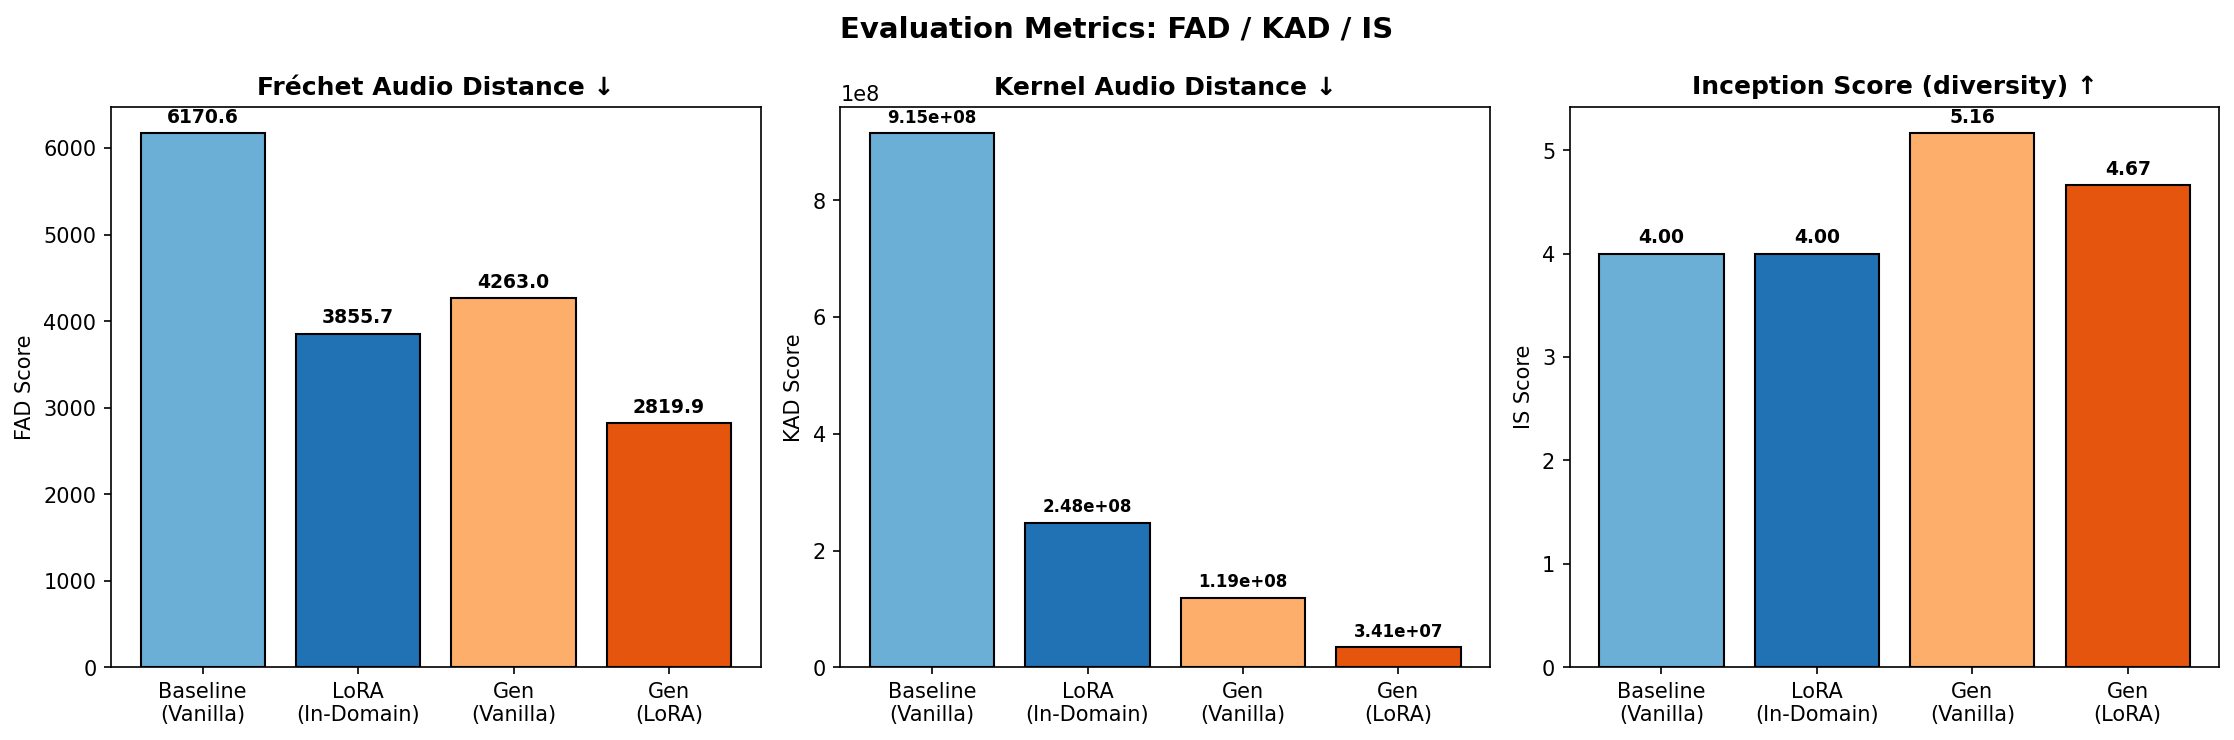
\includegraphics[width=\columnwidth]{fad_kad_is_comparison.png}
\caption{Distributional metrics across configurations. Lower is better
for FAD and KAD; higher is better for the IS proxy.}
\label{fig:fadkad}
\end{figure}

\subsection{Spectral Analysis}

\begin{table}[t]
\centering
\caption{Mean spectral statistics computed with librosa over the
reference set, the vanilla AudioGen baseline, and the LoRA-adapted model
on in-domain prompts.}
\label{tab:spectral}
\setlength{\tabcolsep}{3pt}
\begin{tabular}{lrrr}
\toprule
Feature                     & Reference & Baseline & LoRA \\
\midrule
Spectral centroid (Hz)      & 1511 & 1528 & 1632 \\
Spectral bandwidth (Hz)     & 1239 & 1840 & \textbf{1456} \\
Spectral rolloff (Hz)       & 2828 & 3357 & \textbf{3062} \\
Zero-crossing rate          & 0.113 & 0.060 & \textbf{0.132} \\
RMS                         & 0.088 & 0.062 & \textbf{0.083} \\
\bottomrule
\end{tabular}
\end{table}

Table~\ref{tab:spectral} confirms the FAD/KAD trend at the level of
hand-crafted features. The LoRA-adapted output matches the reference
distribution more closely than the baseline on four out of five features:
bandwidth and rolloff move toward the lower-frequency content
characteristic of Minecraft audio, RMS recovers to within $6\%$ of the
reference, and the zero-crossing rate corrects the baseline's
oversmoothed output (0.060 vs.\ a reference 0.113). The centroid moves in
the opposite direction (1528$\to$1632\,Hz, away from the 1511\,Hz
reference) but the change is within the reference's per-clip standard
deviation ($\pm 848$\,Hz).

\begin{figure}[t]
\centering
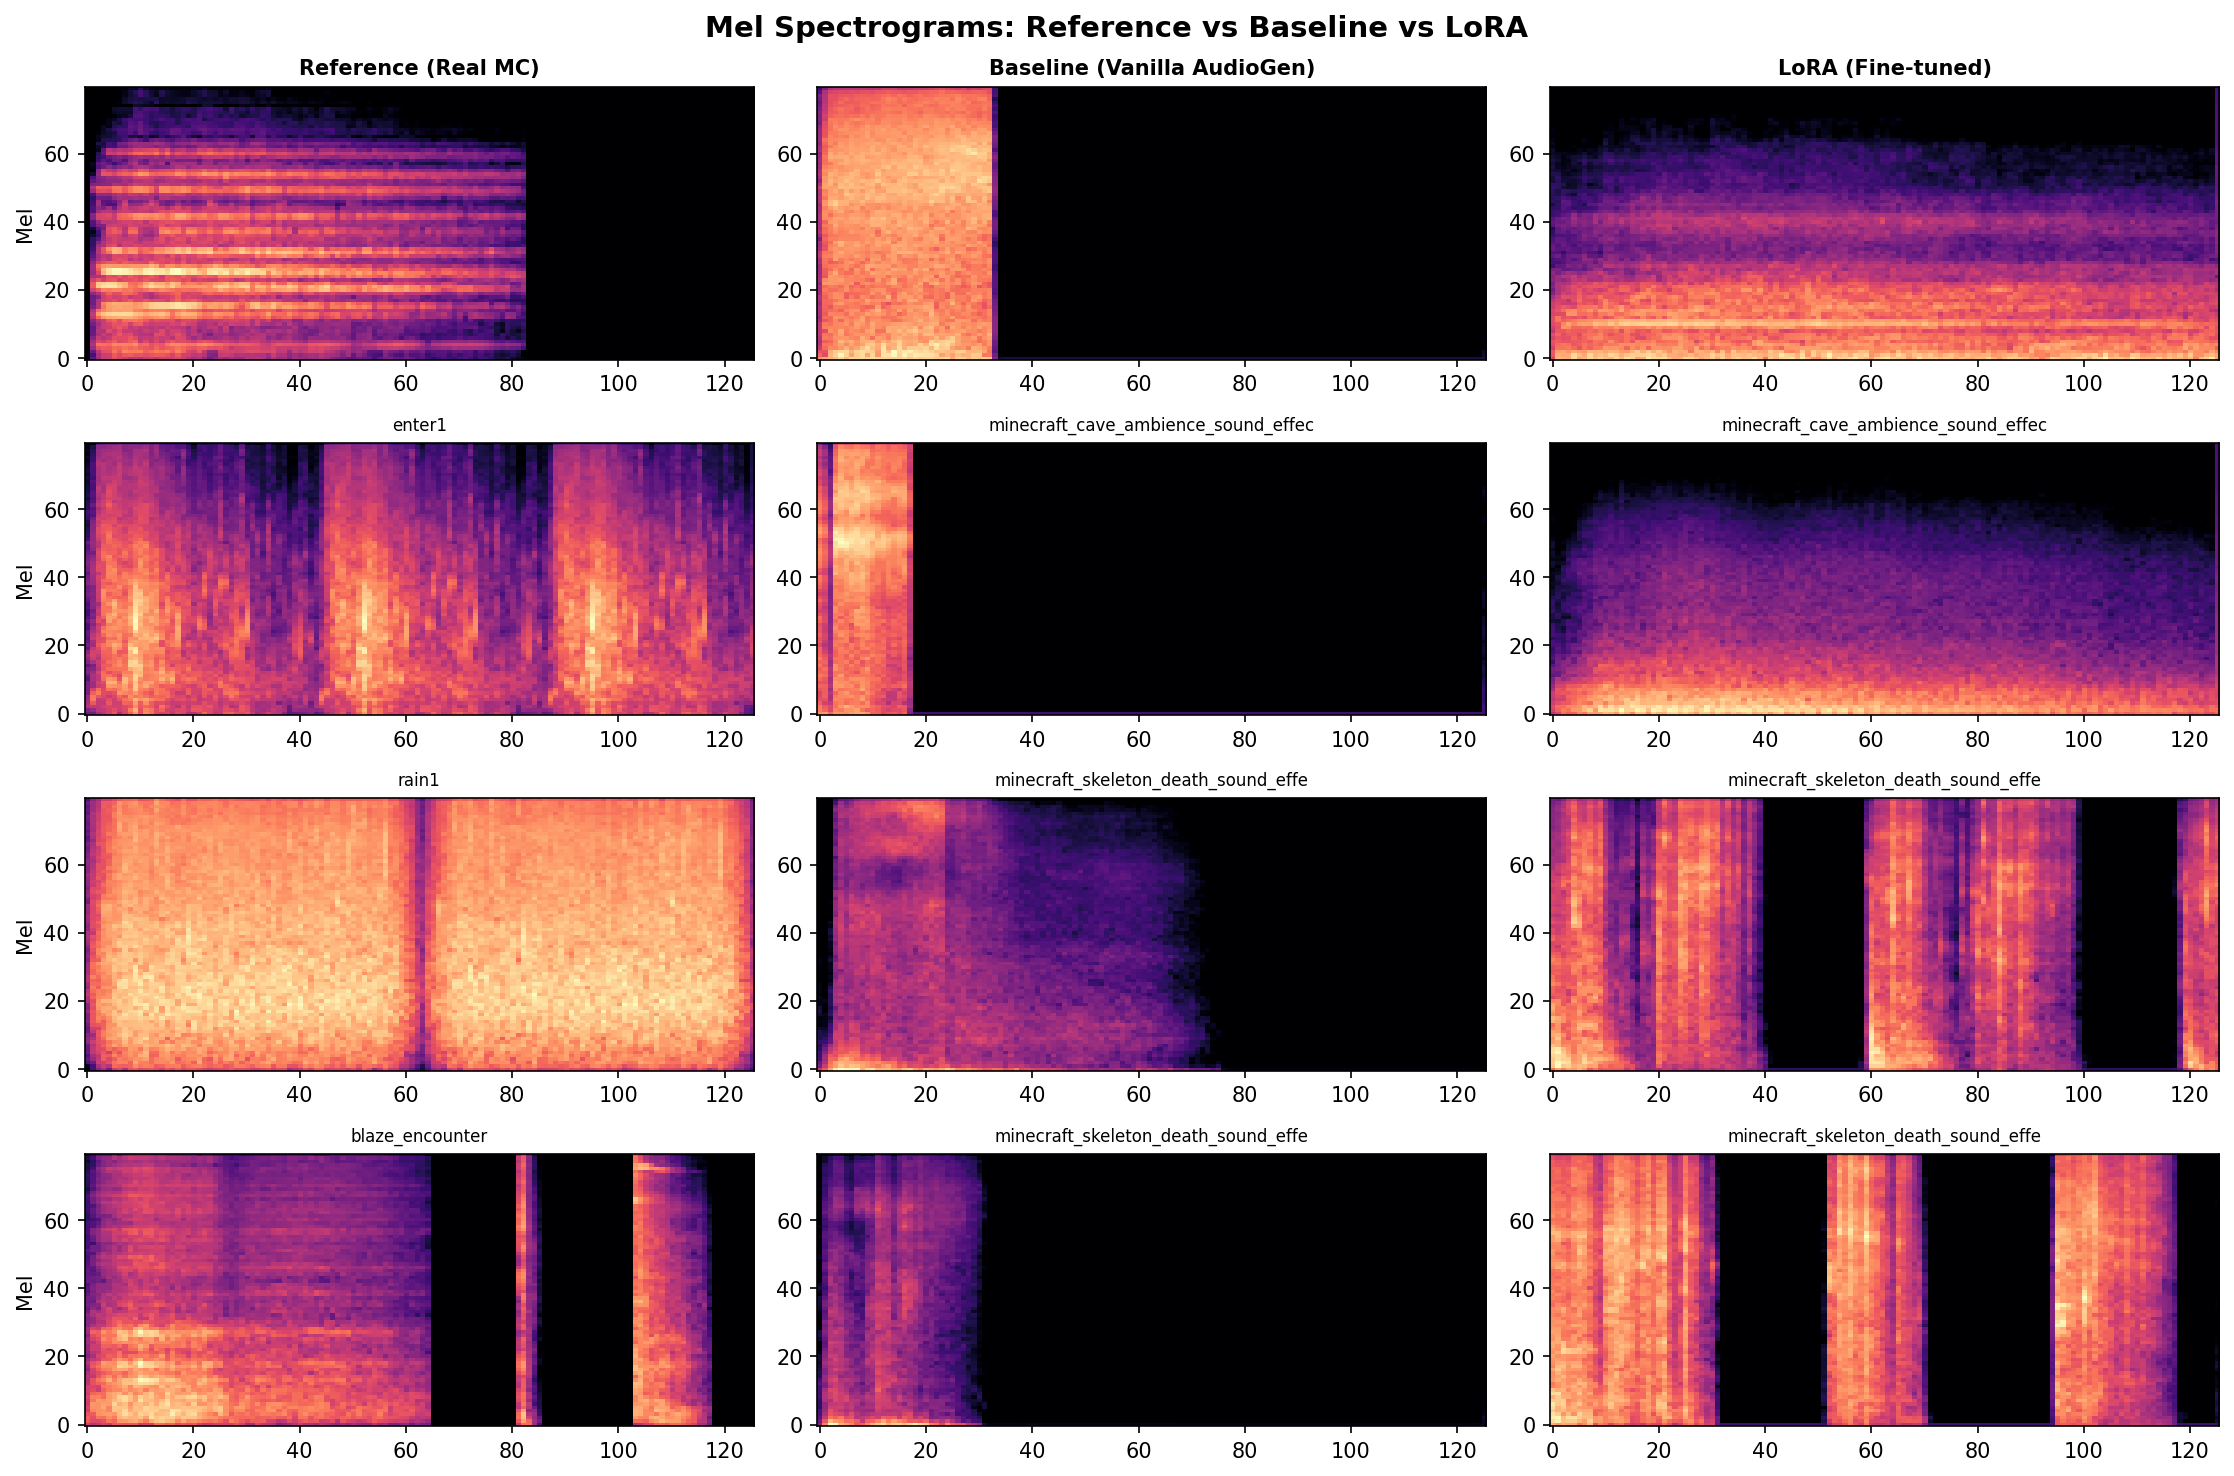
\includegraphics[width=\columnwidth]{spectrogram_3way.png}
\caption{Reference vs.\ vanilla baseline vs.\ LoRA log-power spectrograms
for matched prompts. The LoRA output more closely matches the band-limited,
event-driven structure of the real Minecraft clips.}
\label{fig:spec3way}
\end{figure}

\subsection{Comparison Across Approaches}

LoRA on the AudioLDM\,2 UNet cross-attention produced unstructured noise
after a few hundred optimizer steps; we attribute the failure to
AudioLDM\,2's heterogeneous architecture (CLAP, T5, GPT-2 prefix, UNet,
VAE, and vocoder), which appears to require coordinated adaptation
across several components rather than a single localized adapter on the
UNet. Full fine-tuning of the AudioLDM\,1 UNet for three epochs was
numerically stable but produced only a marginal qualitative
improvement; a longer run on an expanded 556-clip dataset (50 epochs,
roughly 17K steps) converged but did not reach the FAD level of the
AudioGen LoRA. The from-scratch transformer baselines (25\,M
parameters, 50 and 100 epochs) produce intelligible Minecraft-textured
output but lack the prompt-following ability of any of the pretrained
backbones.

\begin{table}[t]
\centering
\caption{Architectural footprint of all six approaches. ``Audio repr.''
is the representation the generative model operates on. Training time is
indicative wall-clock for the 25--100-epoch runs reported here.}
\label{tab:arch}
\setlength{\tabcolsep}{3pt}
\footnotesize
\begin{tabular}{lllll}
\toprule
Approach & Architecture & Base / Trainable & Audio repr. & Time \\
\midrule
AudioLDM\,2 LoRA   & Diffusion (UNet+GPT-2)   & 1.1\,B / $\sim$1\,M LoRA  & Mel spec.   & $\sim$1\,h (T4) \\
AudioLDM Full FT   & Diffusion (all comp.)    & 400\,M / 400\,M (all)     & Mel spec.   & $\sim$2\,h (T4) \\
AudioLDM New Data  & Diffusion (off.\ trainer)& 400\,M / 400\,M (all)     & Mel spec.   & $\sim$8\,h (T4) \\
\textbf{AudioGen LoRA} & \textbf{Autoreg.\ + EnCodec} & \textbf{1.5\,B / 132\,M LoRA} & \textbf{EnCodec tokens} & \textbf{$\sim$3\,h (5090)} \\
From scratch v1    & Custom Tx + T5           & 25\,M / 25\,M (all)       & EnCodec tokens & $\sim$2\,h (T4) \\
From scratch v2    & Custom Tx + T5           & 25\,M / 25\,M (all)       & EnCodec tokens & $\sim$4\,h (T4) \\
\bottomrule
\end{tabular}
\end{table}

\section{Discussion}

\textbf{Why does autoregressive LoRA succeed where diffusion LoRA fails?}
Two factors stand out. First, autoregressive next-token cross-entropy
provides a sharper per-position learning signal than the noise-MSE
objective used in latent-diffusion training, which is particularly
valuable when the dataset is small. Second, the EnCodec discrete token
space is band-limited by construction to the 16\,kHz tokenization grid,
which happens to match Minecraft's lo-fi character; the diffusion latent
of AudioLDM\,2 instead encodes mel-bin reconstructions tuned for
full-bandwidth audio, so adapting it to a low-bandwidth domain requires
moving farther in latent space.

\textbf{The specialisation--generalisation trade-off.}
The OOD CLAP drop ($0.341\to 0.270$) is a direct measurement of the cost
of specialisation. A practitioner facing this trade-off has two
levers: (i) reduce LoRA rank or train for fewer epochs to remain closer
to the base model's general behaviour, or (ii) keep the adapter at its
current strength and treat it as switchable, applying it only when
domain-typical output is desired. The latter strategy preserves the
base model's general capabilities at no additional storage cost beyond
the adapter.

\textbf{Limitations.} Our evaluation is limited by a small reference set
(325 clips total, 48 in validation), which inflates the variance of
distributional metrics; the absolute FAD/KAD numbers should be read as
\emph{relative} comparisons within this study rather than as
cross-paper-comparable scores. We also did not run formal listening tests.

\section{Conclusion}

We presented a domain-specialised text-to-audio system for Minecraft
sound effects. After comparing six adaptation strategies, a
132\,M-parameter LoRA adapter on the autoregressive language model of
AudioGen emerged as the clear winner, reducing FAD by 37\,\% and KAD by
73\,\% versus the vanilla model on in-domain prompts and improving them
further on out-of-distribution multi-event prompts. The negative results
obtained from diffusion-based adaptation and small from-scratch
transformers together support the broader conclusion that, for small
low-fidelity sound domains, autoregressive token models combined with
low-rank adaptation are a more data-efficient choice than fine-tuning a
diffusion-based backbone.

\bibliographystyle{IEEEtran}
\bibliography{refs}

\end{document}
